\section{Preliminaries}
For $m,n,r\in\bbN$ we write $m =_r n$ iff $m=n$ or $m,n>r$.

\subsection{Graphs}
Let $\frakG=(V,E)$ be a graph (possibly with some constants $c_1,\dots,c_n\in V$). 
For $u,v\in V$ we denote by $d^\frakG(u,v)$ the length of a shortest path from $u$ to $v$, where we set $d(u,v) = \infty$ whenever $u$ and $v$ are not connected in $\frakG$.
For $A\subseteq V$ we denote by $\frakG_{\upharpoonright A}$ the induced subgraph of $\frakG$ with vertex set $A$. 
For a nonempty set $A\subseteq V$ and $r\in \bbN$ let $\calN_r^\frakG(A)$ denote the \emph{$r$-neighborhood} of $A$ (and the constants $c_1,\dots,c_n$) in $\frakG$, that is $\frakG_{\upharpoonright\{u\in V\mid \min\{d(u,v) \mid v\in A\cup\{c_1,\dots,c_n\}\} \leq r \}}$.
For a tuple $\vec{u} = (u_1,\ldots, u_k) \in V^k$ we will also write $\calN^\frakG_r(\vec{u})$ instead of $\calN^\frakG_r(\{u_1,\ldots, u_k\})$.

\subsection{Combinatorics on Words}
Let $\Sigma$ be an alphabet. We use $\preceq$ to denote the \emph{prefix-relation} and $\sqsubseteq$ for the \emph{suffix-relation} on $\Sigma^\ast$.  If $u= vw$ we write $v^{-1}u = w$ and
$uw^{-1} = v$.
Let $\pref_r(u)$ denote the maximal prefix of $u$ of length at most $r$. For $u,v\in\Sigma^\ast$ let $u \sqcap v$ denote the largest suffix of $u$ that is also a prefix of $v$.

In a first lemma we prove that the complementary prefix and suffix of $u$ resp.~$v$ wrt.~$u\sqcap v$ can be shortened to words of length at most $2r$ having the same prefixes and suffixes:

\begin{lemma}\label{lem:short_ends_construction}
	Let $r\in\bbN$ and $u,v,w \in\Sigma^\ast$ with $uw\sqcap wv = w$. %such that the period of $w$ has length at least $2$. 
	Then there are words $u',v'$ of length $\calO(r)$ such that 
	\begin{itemize}
		\item $\suf_r(uw) = \suf_r(u'w)$,
		\item $\suf_r(wv) = \suf_r(wv')$,
		\item $\pref_r(wv) = \pref_r(wv')$,
		\item $u'w\sqcap wv' = w$.
	\end{itemize}
\end{lemma}
\begin{proof}
	Set $u'=\suf_r(u)$. Additionally, if $|v|\leq 2r$ set $v':=v$, and otherwise, set $v':=\pref_r(v)\suf_r(v)$. Then the first three equations are obviously satisfied. Now assume $u'w\sqcap wv'\neq w$, i.e., there is $w'\in \Sigma^*$ with $|w'|>|w|$, $w'\preceq wv'$, and $w'\sqsubseteq u'w$. Since $|u'w|\leq r+|w|$ we have $w'\preceq w\pref_r(v)\preceq wv$. Additionally, we have $w'\sqsubseteq u'w\sqsubseteq uw$ implying $|uw\sqcap wv|\geq|w'|>|w|$. This is a contradiction to the definition of~$w$.
\end{proof}

A \emph{period} of a word $u$ is a word $v$ such that $u \preceq v^\omega$. Obviously every word $u$ has a unique smallest period, which we denote by $\root{u}$. The \emph{left-exponent} of $u$ in $v$ is the largest number $n$ such that $v= u^nw$, and it is denoted by $\lexp(u,v)$. The \emph{right-remainder}, $v\mod u$,  of $v$ with respect to $u$ is defined as $(u^{\lexp(u,v)})^{-1}v$, that is the unique $w$ such that $v= u^{\lexp(u,v)}w$.  In particular we have $v= \root{v}^{\lexp(\root{v}, v)}(v \mod \root{v})$ for every $v\in\Sigma^\ast$. A word $u$ is \emph{primitive} if there is no $v$ with
$|v| < |u|$ and $u = v^n$ for some $n\in\bbN$.
For $u,v\in\Sigma^\ast$ let $u\Delta v = (y,z)$, where $y,z$ are minimal such that there exists an $x$ with $u=xy$ and $v=xz$. For $\bar{v}, \bar{w}\in(\Sigma^\ast)^k$ let 
$\bar{v}\Delta\bar{w} = (v_1\Delta w_1,\ldots, v_k\Delta w_k) \in (\Sigma^\ast)^{2k}$ and $|\bar{w}| \coloneq \sum_{i=1}^{k}|w_i|$. 

\begin{definition}
	Let $u\in \Sigma^\ast$ be a word. A \emph{canon-decomposition} of $u$ is a sequence of words $\epsilon = u_0,u_1,\ldots, u_n = u$ such that for all $0\leq i < n$ it holds that
	$u_i \precneq u_{i+1}$ and $u_i \sqsubsetneq u_{i+1}$ ($u_i \presuf u_{i+1}$ for short). A canon-decomposition $u_0,u_1,\ldots, u_n $ is \emph{complete} if there is no $1\leq i< n$ and $v\in\Sigma^\ast$ with $u_i \presuf v \presuf u_{i+1}$.
\end{definition}

\begin{lemma}
	Every word $w\in\Sigma^\ast$ has a unique complete canon-decomposition.
\end{lemma}
\begin{proof}
	Obviously, every word $w$ possesses at least one complete canon-decomposition. Now suppose $\vec{u} = (u_0,\ldots,u_m)$ and $\vec{v}=(v_0,\ldots,v_n)$ are two distinct complete canon-decompositions of
	a word $w\in\Sigma^\ast$. W.l.o.g. assume that $n \leq m$. We claim that there is an $0\leq i \leq n$ with $u_i \neq v_i$. Because otherwise it follows from $w= u_n = v_n$ that    
	$\vec{u}$ and $\vec{v}$ have the same length $n$ and this, in turn, implies that they are identical since $u_i=v_i$ for all $0\leq i\leq n$. Now choose the smallest $i$ between $0$ and $n$ such that $u_i \neq v_i$. As $u_0 = \epsilon = v_0$ it holds that $i>0$. Hence $u_{i-1}, v_{i-1}$ are defined and $u_{i-1} = v_{i-1}$. Since $u_i, v_i \preceq w$ and $u_i \neq v_i$ it must be the case that $|u_i| \neq |v_i|$. Again w.l.o.g. assume that $|u_i| < |v_i|$. Then  $u_i, v_i \preceq w$, $u_i, v_i \sqsubseteq w$ and $|u_i| < |v_i|$, which implies $u_i \presuf v_i$. Therefore 
	$v_{i-1} = u_{i-1} \presuf u_i \presuf v_i$ in contradiction to the completeness of $\vec{v}$!
\end{proof}

\begin{example}
	The  complete canon-decomposition of $ababa$ is $(\epsilon, a, aba, ababa)$.
\end{example}

%\begin{definition}
%	A word $u$ is \emph{periodic} if $u=v^n$ for some $v\in\Sigma^+$ and $n>1$. Otherwise $u$ is primitiv. We say that $u$ is almost periodic if $u= (vw)^nv$ for some $n\geq 1$,  $v\in \Sigma^\ast$, and $w\in\Sigma^+$.  We write $\sqrt{u}^{\ast}$ for the unique pair $(v,w) \in \Sigma^\ast\times\Sigma^+$ such that
%   $vw$ is primitive and $u = (vw)^nv$ for some $n\geq 1$.
%
%\end{definition}

%\begin{lemma}
%	Let $\vec{u} = (u_0,\ldots,u_n)$ be a complete canon-decomposition. Then $\root{u_{i+1}} = u_{i+1}u_i^{-1}$ for all $0\leq i < n$. 
%\end{lemma}
%\begin{proof}
%	Fix some $0\leq i < n$ and let $v:= u_{i+1}u_i^{-1}$. Let us verify first that $v$ is indeed a period of $u_{i+1}$. If $2|u_i| \leq |u_{i+1}|$ then $u_{i+1} = u_iwu_i$ for some $w\in\Sigma^\ast$. 
%	Hence $v= u_iw$ and $u_{i+1} \preceq (u_iw)^\omega = v^\omega$. Otherwise  $2|u_i| > |u_{i+1}|$ and therefore the $u_i$-prefix and the $u_i$-suffix of $u_{i+1}$ overlap. We can use this overlap to 
%	show via a simple induction that the situation is as depicted in Fig.~\ref{fig:root}.
%	\begin{figure}[h]
%		\centering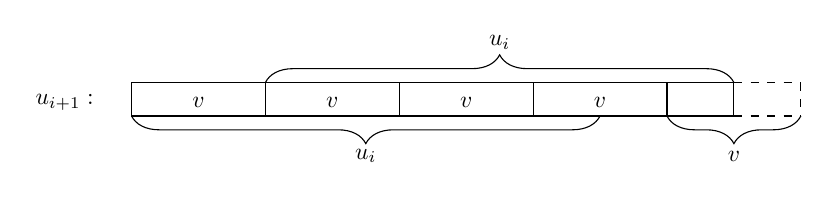
\begin{tikzpicture}[scale=0.85,every node/.style={scale=0.85}]
	\node at (-1, .2) {$u_{i+1}:$};
	\node at (1, .2) {$v$};
	\node at (3, .2) {$v$};
	\node at (5, .2) {$v$};
	\node at (7, .2) {$v$};
	\draw [decorate,decoration={brace,amplitude=10pt}] (10,0) -- (8, 0) node [black,midway,yshift=-.6cm] {$v$};
	\draw (0,0) rectangle (9, .5);
	\draw [decorate,decoration={brace,amplitude=10pt}] (7,0) -- (0, 0) node [black,midway,yshift=-.6cm] {$u_i$};
	\draw [decorate,decoration={brace,amplitude=10pt}] (2,0.5) -- (9, 0.5) node [black,midway,yshift=.6cm] {$u_i$};
	\draw (2,.5) -- (2,0);
	\draw (4,.5) -- (4,0);
	\draw (6,.5) -- (6,0);
	\draw (8,.5) -- (8,0);
	\draw[dashed] (10,.5) -- (10,0);
	\draw[dashed] (9,.5) -- (10,.5);
	\draw[dashed] (9,0) -- (10,0);   
\end{tikzpicture}
%		\caption{\label{fig:root}}
%	\end{figure}
%
%	Now suppose that $|\root{u_{i+1}}| < |v|$. Then let $u_i' \coloneq \root{u_{i+1}}^{\lexp(\root{u_{i+1}}, u_{i+1}) -1}(u_{i+1} \mod \root{u_{i+1}})$.
%	Then $u_i' \presuf u_{i+1}$ and $|u_i'| = |u_{i+1}| - \root{u_{i+1}} > |u_{i+1}| - |v| = |u_i|$. Hence $u_i\presuf u_i' \presuf u_{i+1}$ contradicting the completeness of $\vec{u}$! 
%\end{proof}

From the complete canon-decomposition of a word~$w$ we derive the so called skeleton of~$w$ containing the inner words $v$ of all canons $uvu$ in $w$.

\begin{definition}
	Let $w\in\varSigma^\ast$ and $\vec{w} = (w_0,\ldots,w_n)$ be the complete canon-decomposition of $w$. The \emph{$r$-skeleton} of $w$, denoted by $\calS_r(w)$, is the word of length $n$ over the alphabet $\Gamma = \Sigma^{\leq r}$ with $\calS_r(w)[i] = \pref_r(w_i^{-1}w)$ for each $0\leq i\leq n-1$. Note that $w_i^{-1}w_{i+1}$ is always defined since $w_i\preceq w$.
\end{definition}

\begin{example}
	Let $u= bababa$ and $v=ababab$. Then $u\sqcap v = ababa$ and the complete canon-decomposition of $u\sqcap v$ is $(\epsilon, a, aba, ababa)$. The $2$-skeleton of $(u,v)$ is the word depicted below.
	\begin{center}
		\begin{tikzpicture}[scale=0.85]
		\node[] (0) {$ab$};
		\node[ right=of 0] (1) {$ba$};
		\node[ right=of 1] (2) {$ba$};
		
		\path[ ->,>=latex'] (0) edge (1)
		(1) edge (2);
		\end{tikzpicture}
	\end{center}
\end{example}

By definition the $i$-th element of the canon decomposition of  $u\sqcap v$ corresponds to the $i$-th letter of the skeleton. We will use this correspondence to translate back and forth between 
an Ehrenfeucht-Fra\"{\i}ss\'{e} game played on the Cayley-graph of a queue monoid and games played on certain skeletons which are derived from the game played on the Cayley-graph. 

\begin{lemma}\label{lem:short_from_skeleton}
	Let $r\in\bbN$, $w\in\Sigma^*$ and $n\in\bbN$ be the length of $\calS_r(w)$. Then a word $v\in\varSigma^*$ can be contructed from $w$ such that $|v|=\calO(2^{n\cdot r})$ and $\calS_r(w)=\calS_r(v)$.
\end{lemma}
\begin{proof}
	Let $\vec{w}=(w_0,\dots,w_n)$ be the complete canon-decomposition of~$w$. At first, assume $|\calS_r(w)[n-1]|<r$ (i.e., the last component is small). Then there are two possibilities: on the one hand $w=w_{n-1}xw_{n-1}$ and $|xw_{n-1}|<r$. In this case we have $|w|<2r=\calO(3^{nr})$. On the other hand there could be $w_i$ and $k\in\bbN$ such that $w=w_i^k$ and $w_{n-1}=w_i^{k-1}$. But then we have $|w_i|<r$ and $|w|<kr\leq nr=\calO(3^{nr})$. So, from now on we may assume $|\calS_r(w)[n-1]|=r$.
	
	We construct~$v$ inductively as follows: We set $v_0:=\epsilon$. Now let $a,b\in\varSigma^*$ be distinct with $\calS_r(w)[0]\in a\varSigma^*$. Then $x\presuf\calS_r(w)[0]b^r$ implies $x=\epsilon$ or $x=\calS_r(w)[0]b^r$. Hence, we set $v_1:=\calS_r(w)[0]\,b^r$. Additionally, for $1\leq i<n$, set $v_{i+1}:=v_i\,\calS_r(w)[i]\,a^ib^{r}v_i$. Finally, we set $v:=v_{n}$. Thereby, $v$ is called the \emph{canonical $r$-instantiation of $\calS_r(w)$}.
	
	At first, we observe $\root{v_{i+1}}=v_i\,\calS_r(w)[i]\,a^ib^{r}$ for each $1\leq i\leq n$: This is easy to see, since in $v_i$ there is an alternation of words of increasing length (these are $\calS_r(w)[j]a^j$) and blocks $b^r$.
	
	Additionally, by construction $\vec{v}=(v_0,\dots,v_{n})$ is a canon-decomposition of~$v$. Next, we prove by induction that $(v_0,\dots,v_{i+1})$ is a complete canon-decomposition of~$v_i$ for each $0\leq i<n$. The case $i=0$ is obvious by definition of~$v_1$. So, let $1\leq i\leq n$. Assume there is $u\in\varSigma^*$ with $v_i\presuf u\presuf v_{i+1}$. Then there are two possible cases:
	
	First, assume $v_i\,\calS_r(w)[i]\,a^ib^{r}\preceq u$ (cf.\ Fig~\ref{fig:skeleton}). Let $s$ be the complementary suffix wrt.~$u$. But then $\calS_r(w)[i]\,a^ib^{r}s$ is also a suffix of $v_i$ - contradicting the construction of~$v_i$ to not contain $\calS_r(w)[i]\,a^ib^r$.
	
	\begin{figure}[h]
		\centering\begin{tikzpicture}[scale=0.85,every node/.style={scale=0.85}]
	\node at (-0.75,0.2){$v_{i+1}=$};
	\node at (-0.75,-1.4){$u=$};
	\node at (-0.75,-2.2){$u=$};
	
	\draw (0,0) rectangle (15,0.75);
	\draw (0, -1) rectangle (10,-1.75);
	\draw (5, -1.75) rectangle (15,-2.5);
	
	\draw (6,.75) -- (6,0);
	\draw (7.5,.75) -- (7.5,0);
	\draw (9,.75) -- (9,0);
	
	\node at (6.8,0.35) {$\mathcal{S}_r(w)[i]$};
	\node at (8.25,0.35) {$a^ib^r$};
	
	\draw (6,-1) -- (6,-2.5);
	\draw (7.5,-1) -- (7.5,-2.5);
	\draw (9,-1) -- (9,-2.5);
	\draw (11,-1.75) -- (11,-2.5);
	\draw (12.5,-1.75) -- (12.5,-2.5);
	\draw (14,-1.75) -- (14,-2.5);
	\draw (11,0) -- (11,0.75);
	\draw (12.5,0) -- (12.5,.75);
	\draw (14,0) -- (14,.75);
	
	\node at (6.8,-1.4) {$\mathcal{S}_r(w)[i]$};
	\node at (6.8,-2.2) {$\mathcal{S}_r(w)[i]$};
	\node at (8.25,-1.35) {$a^ib^r$};
	\node at (8.25,-2.15) {$a^ib^r$};
	\node at (11.8,-2.2) {$\mathcal{S}_r(w)[i]$};
	\node at (13.25,-2.15) {$a^ib^r$};
	\node at (11.8,0.35) {$\mathcal{S}_r(w)[i]$};
	\node at (13.25,0.35) {$a^ib^r$};
	
	\draw[->,>=latex'] (6.75,-0.1) -- (6.75,-0.9);
	\draw[->,>=latex'] (8.25,-0.1) -- (8.25,-0.9);
	\draw[->,>=latex'] (9.1,-2.125) -- (10.9,-2.125);
	\draw[->,>=latex'] (11.75,-1.65) -- (11.75,-0.1);
	\draw[->,>=latex'] (13.25,-1.65) -- (13.25,-0.1);
	
	\draw[snake=brace] (0,0.8) -- (6,0.8);
	\draw[snake=brace] (9,0.8) -- (15,0.8);
	
	\node at (3,1.1) {$v_i$};
	\node at (12,1.1) {$v_i$};
\end{tikzpicture}
		\caption{\label{fig:skeleton}}
	\end{figure}
	
	Second, assume $u\precneq v_i\,\calS_r(w)[i]\,a^ib^{r}$. Let $s$ be the complementary suffix of~$u$. Then it is easy to see that $s$ is a period of $v_i$. Hence, we have $s=v_{i-1}\,\calS_r(w)[i-1]\,a^{i-1}b^{r}$, which is a contradiction, again.
	
	Hence, $\vec{v}$ is a complete canon-decomposition of~$v$. Finally, let $0\leq i<n$. Then we have
	\[\calS_r(v)[i]=\pref_r(\inv{v_i}v)=\pref_r(\calS_r(w)[i]\,s)=\calS_r(w)[i]\]
	for some $s\in\varSigma^*$, i.e., $\calS_r(v)=\calS_r(w)$.
\end{proof}